\documentclass{beamer}
\usepackage{ dsfont }
\usepackage[utf8]{inputenc}
\usepackage[english]{babel}
\setbeamersize{text margin left=10pt, text margin right=10pt} %new code
\usepackage{graphicx}
\usepackage{float}
\usepackage{subcaption}

\usepackage{animate}
\usepackage{movie15}
\usepackage{breqn, bm}
\usepackage{tcolorbox, amsmath}
\usepackage{subcaption}

\definecolor{notgreen}{RGB}{255,127,0}
\definecolor{green}{RGB}{49,150,3}
\setbeamerfont{headline}{size=\small}


%----------------------------------------------------------------------------------------
%	 Package
%----------------------------------------------------------------------------------------
\usepackage{color}
\usepackage{url}
\beamertemplatenavigationsymbolsempty
\definecolor{cadmiumred}{rgb}{0.8, 0.8, 0.8}

%----------------------------------------------------------------------------------------
%	 Presentation settings
%----------------------------------------------------------------------------------------

\usetheme{Madrid}
\usecolortheme{beaver}

\setbeamertemplate{itemize items}[triangle] 
\setbeamertemplate{enumerate items}[default]
 
\title[ML in Music]{
	Machine Learning, Advanced Topics, 6th Seminar\\ 
	\vspace{1cm}
	\textbf{\textcolor{black}{Application of Modern Machine Learning in Music  }}}

\author{Valentin Malykh}
\institute[MIPT]{
	Moscow Institute of Physics and Technology\\
	
	\medskip
	
	\textbf{mail}: \href{mailto:valentin.malykh@phystech.edu}{\textcolor{blue}{\nolinkurl{valentin.malykh@phystech.edu}}}
		
}
	

\date{\today}

\newcommand{\Expect}{\mathsf{E}}
\newcommand{\MExpect}{\mathsf{M}}
\newcommand{\cov}{\mathsf{cov}}
\setbeamertemplate{section in toc}[circle]


\begin{document}
\begin{frame}
	\titlepage 
\end{frame}

\begin{frame}{How to apply ML for Music Data to get Money?} 
	\begin{itemize}
		\item You are working in a big music service as a data scientist
		\begin{center}		  
		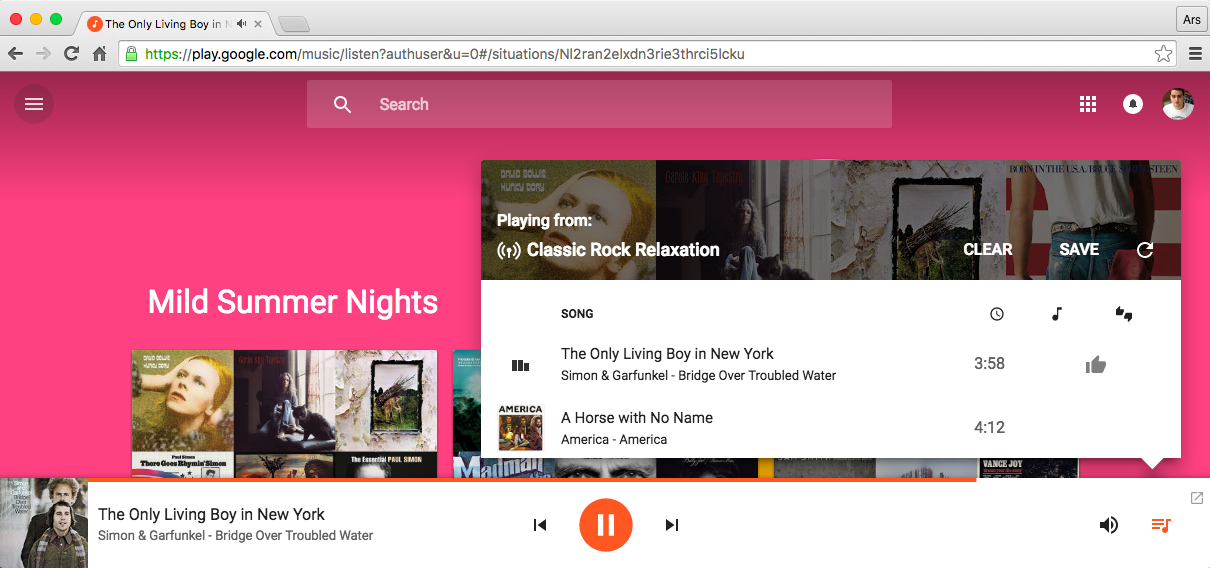
\includegraphics[scale=0.15]{img/interface}~~~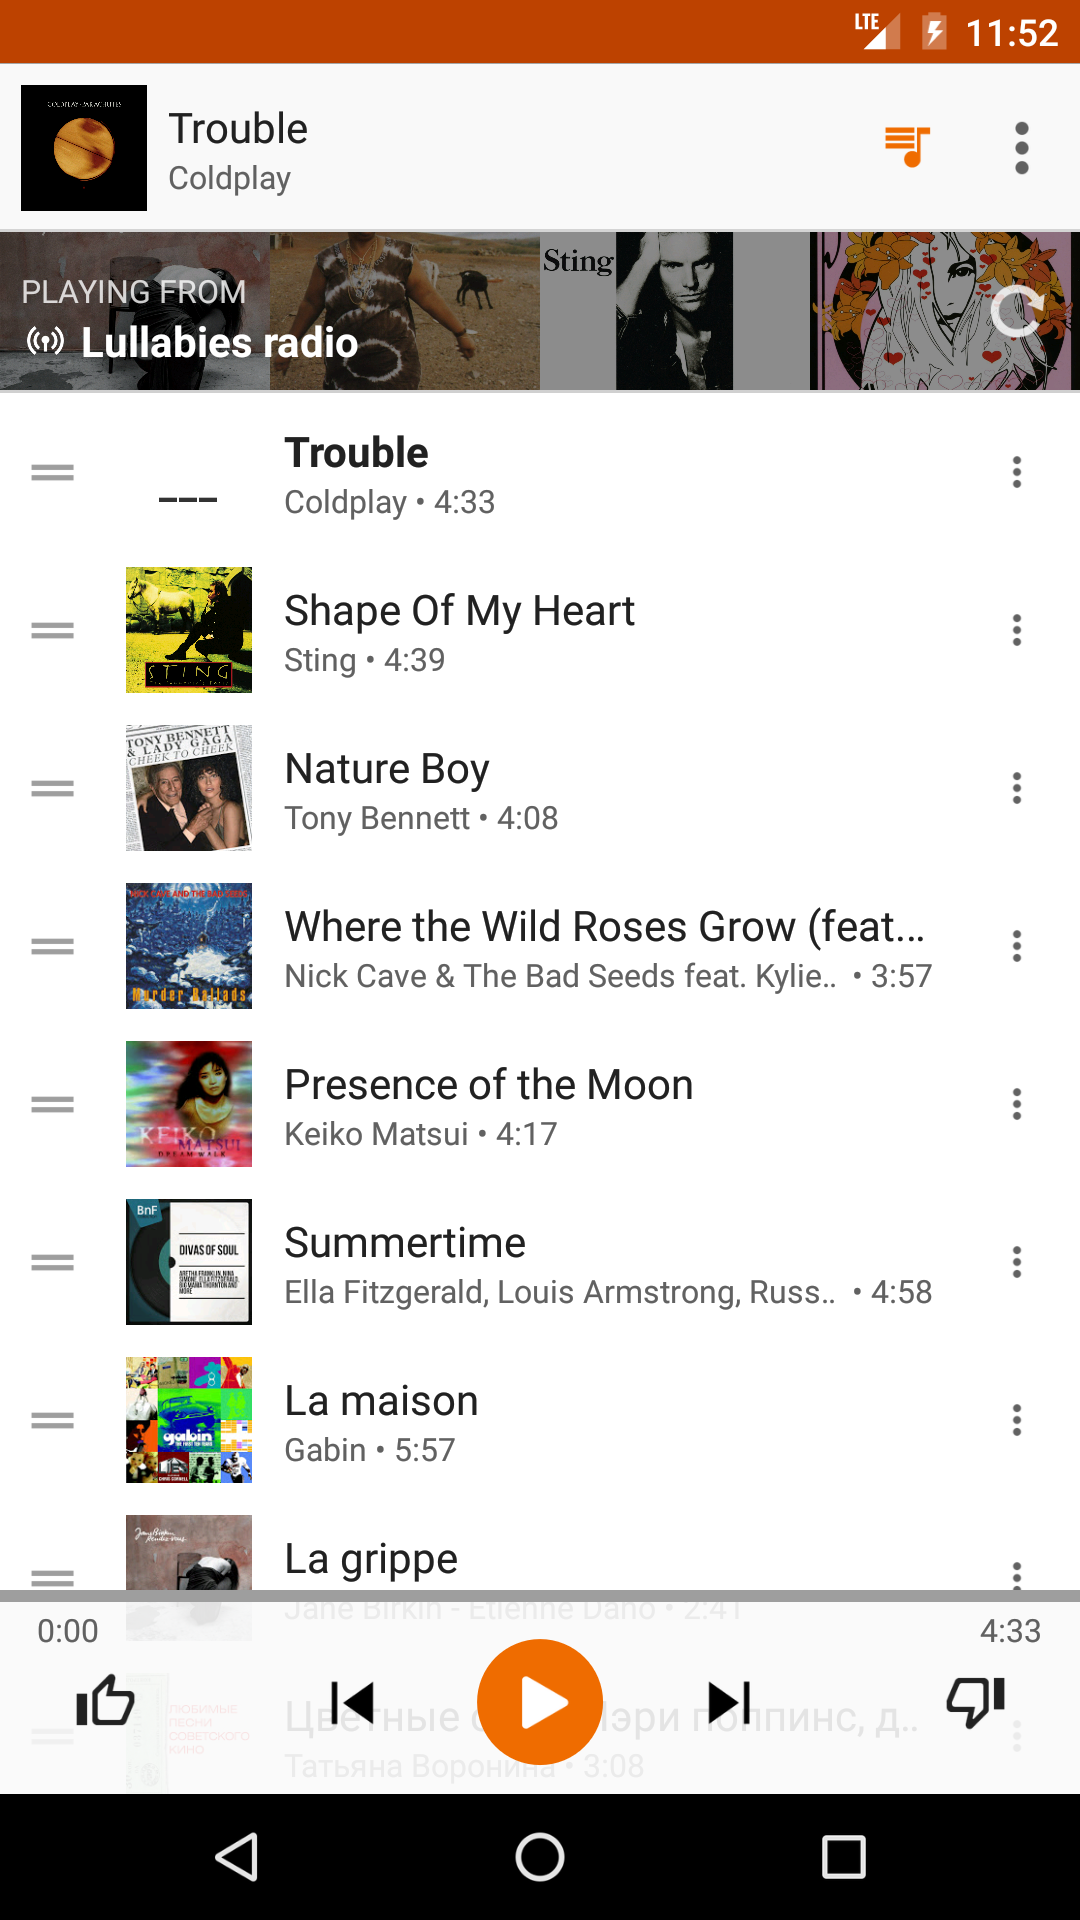
\includegraphics[scale=0.044]{img/phone}
		\end{center}
		\item In this service there's a lot of music data -- mp3 files
			\begin{center}
			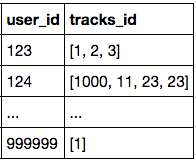
\includegraphics[scale=0.4]{img/u2t}~~~~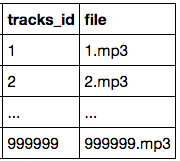
\includegraphics[scale=0.4]{img/t2f} 
			\end{center}
		\item You were given the task -- make money using this data
	\end{itemize}
\end{frame}

\begin{frame}{What is the sound?} 
	\begin{itemize}
		\item Waves and Recording
			\begin{center}		  
				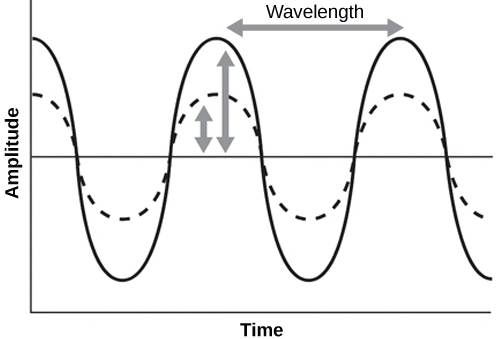
\includegraphics[scale=0.25]{img/wave} ~~~ 	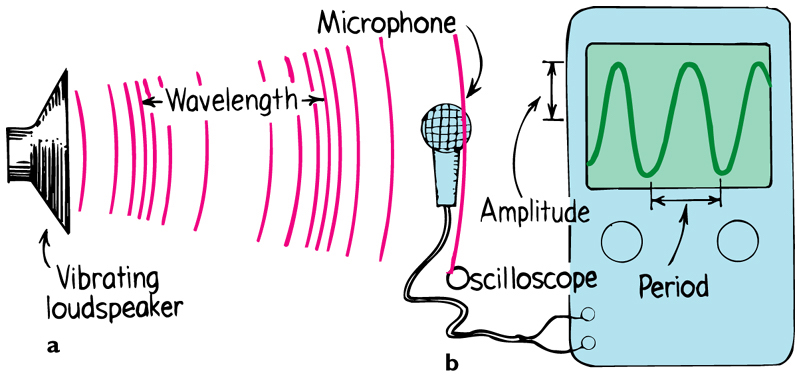
\includegraphics[scale=0.2]{img/sound}
			\end{center}
		\item How to store sound? Store as huge array with samples.
		\begin{center}
			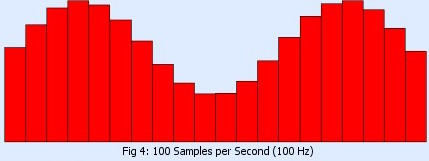
\includegraphics[scale=0.35]{img/sf1}~~~~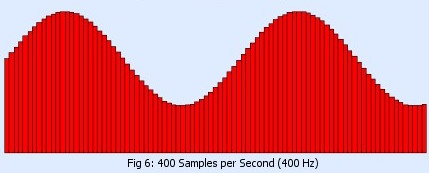
\includegraphics[scale=0.35]{img/sf2} 
		\end{center}
		\item $[1, 2, 3, 5, 3, 2, 1, 1, 1, 1, 2, 3, 5, 3, 2]$, Usually 16 000 float per second
	\end{itemize}
\end{frame}

\begin{frame}{Finding similar tracks}
	\begin{itemize}
		\item How to find similar tracks using ML methods?
			\begin{center}		  
				\textcolor{blue}{Data}: 30 sec * 16000 features, $10^7$ items
				
				\textcolor{red}{Task}: define function of $similarity(track_i, track_j)$
			\end{center}
		
		\item  Why ordinary methods are so bad?
			\begin{itemize}
				\item shift and noise tolerance, over-fitting 
			\end{itemize}
		
		\item Metric approach is still good idea, if we have a high level description
		\item Good representation of music track
		\begin{itemize}
			\item Human -- guitar, rock, Queen, 1997, UK, 3 min., .... 
			\item Computer -- good small vector of numbers  
		\end{itemize}
		
			\begin{center}
				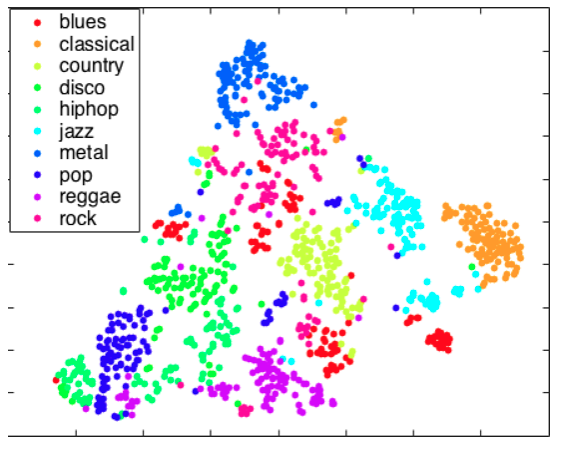
\includegraphics[scale=0.2]{img/geners}
			\end{center}
		
	\end{itemize}
\end{frame}


\begin{frame}{Get good representation using Convolutional Neural Nets}
	\begin{center}
		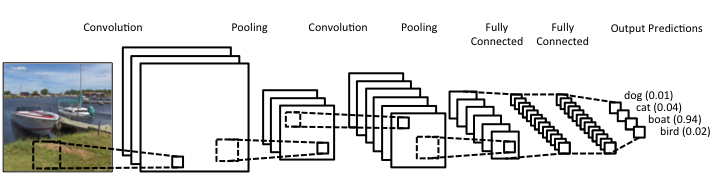
\includegraphics[scale=0.4]{img/cnn}
		
		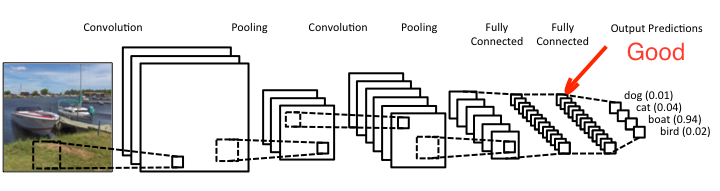
\includegraphics[scale=0.4]{img/cnn_gr}
	\end{center}
	
	\begin{tcolorbox}[colback=gray!2, colframe=red!90, title=Issue]
		\centering We need to get picture!
	\end{tcolorbox}
\end{frame}

\begin{frame}{What is the sound? (2)} 
	We have some wave 
	
		\begin{center}
			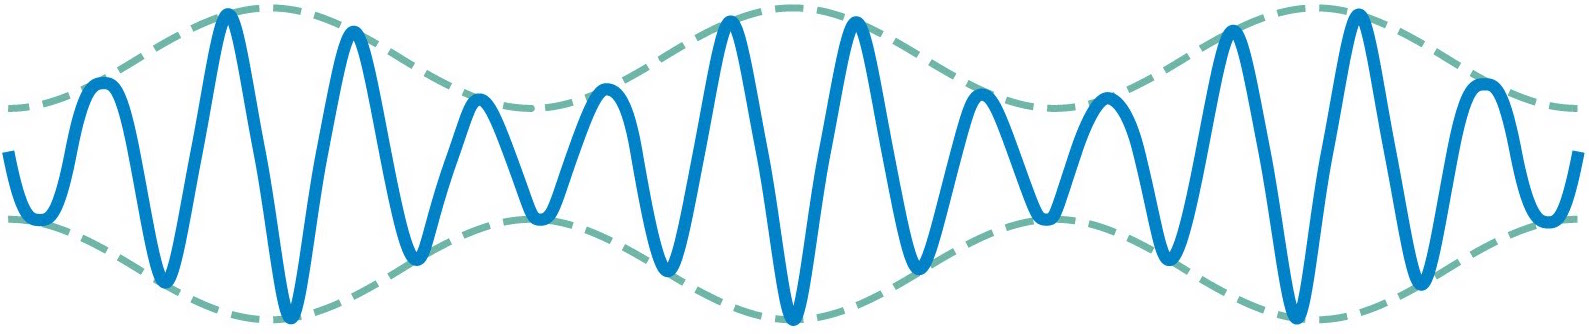
\includegraphics[scale=0.1]{img/wave1}
		\end{center}
		
	lets represent this wave as a sum of two waves 
	
		\begin{center}
			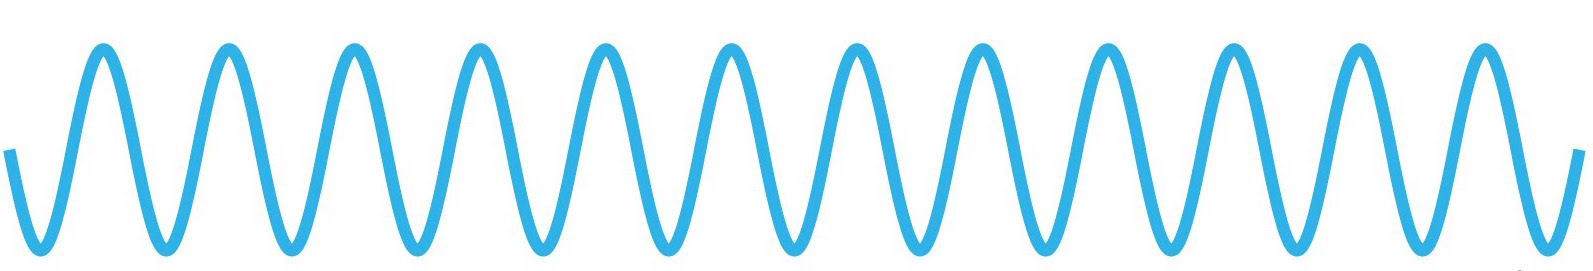
\includegraphics[scale=0.1]{img/wave2}
			
\includegraphics[scale=0.1]{img/wave3}
		\end{center}
	
	sound is a combination of big waves range
	
		\begin{center}
			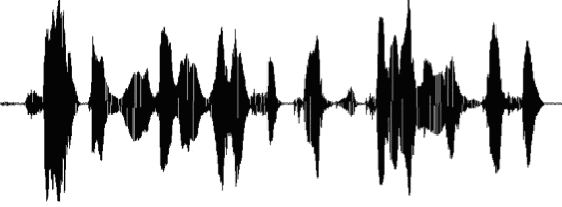
\includegraphics[scale=0.4]{img/sound_}
		\end{center}
	
	\begin{center}
		What have we lost in our representation?
	\end{center}	
\end{frame}

\begin{frame}{Getting the Frequency} 
	\begin{center}
		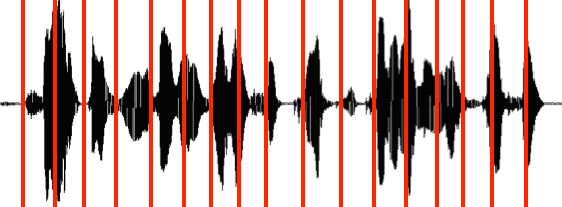
\includegraphics[scale=0.5]{img/sound_sl}
		
		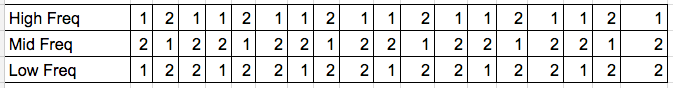
\includegraphics[scale=0.4]{img/hist}~~~~~~~~
		
		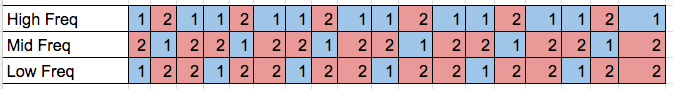
\includegraphics[scale=0.4]{img/histc}~~~~~~~~~
		
		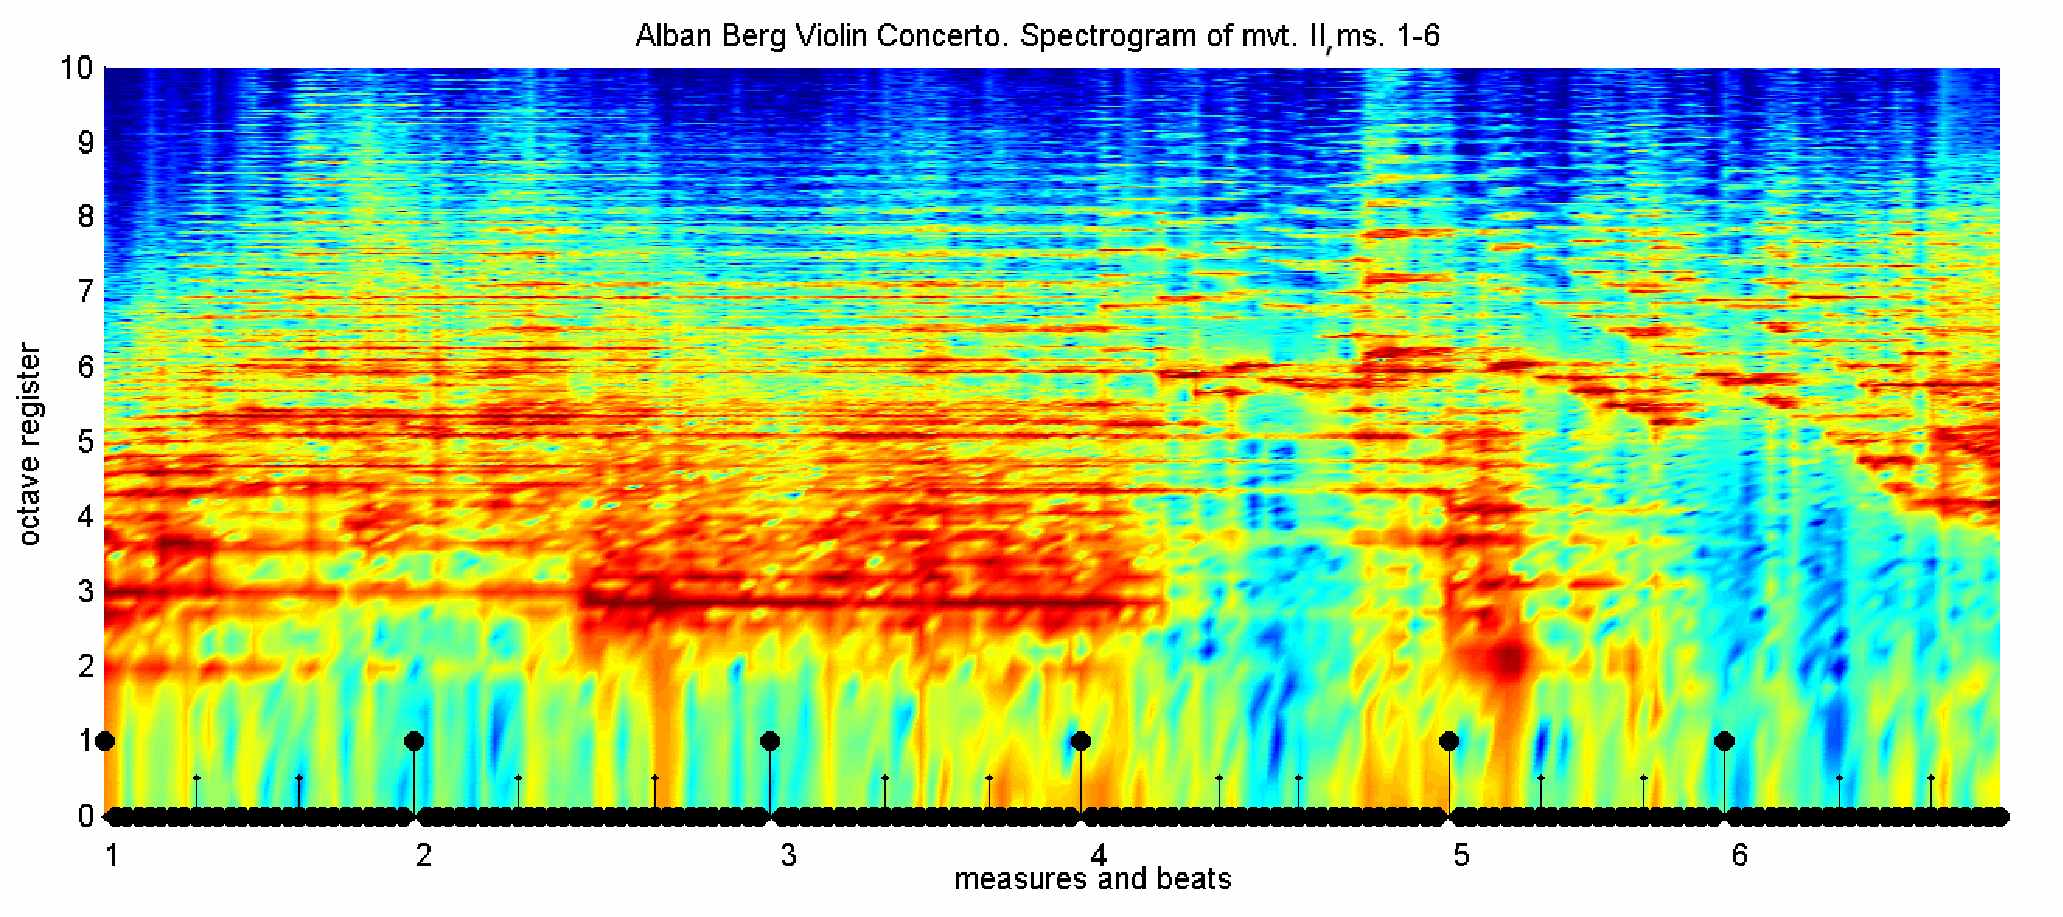
\includegraphics[scale=0.3]{img/spect}~~~~~~~~~
	\end{center}
	
\end{frame}


\begin{frame}{We need to train Neural Nets, but how can we do that?!}
	\begin{itemize}
		\item But how can we train the nets on music? 
		\item Let's invent a fake machine learning task

		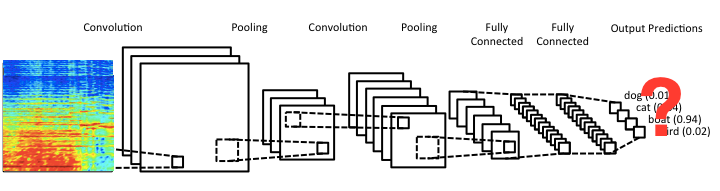
\includegraphics[scale=0.4]{img/cnn_what2predict}~~~~~~~~~

		\begin{itemize}
			\item genre classification
			\item artist classification
			\item rating prediction
			\item .....
		\end{itemize}
	\end{itemize} 
	
\end{frame}

\begin{frame}{Fully connected NN} 
		\begin{center}
			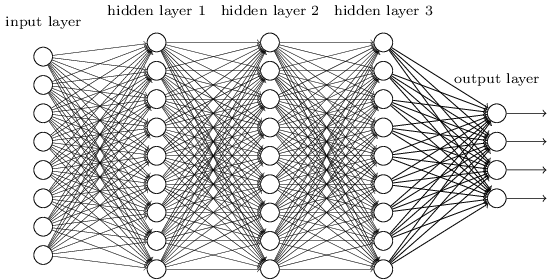
\includegraphics[scale=0.5]{img/fc}
		\end{center}
		\begin{itemize}
			\item too many parameters -- number of weights = $16^4 * neurons$ + ... 
			\item It doesn't work =( 
		\end{itemize}
\end{frame}

\begin{frame}{Convolution NN} 
		Let's invent some convolution architecture
		\begin{center}
			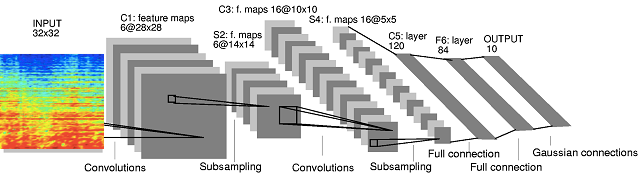
\includegraphics[scale=0.5]{img/conv}
		\end{center}
		important detail -- pooling of time axis \href{http://bit.ly/1slJTgi}{[\textcolor{green}{Spotify} Deep Learning]}
		\begin{center}				
			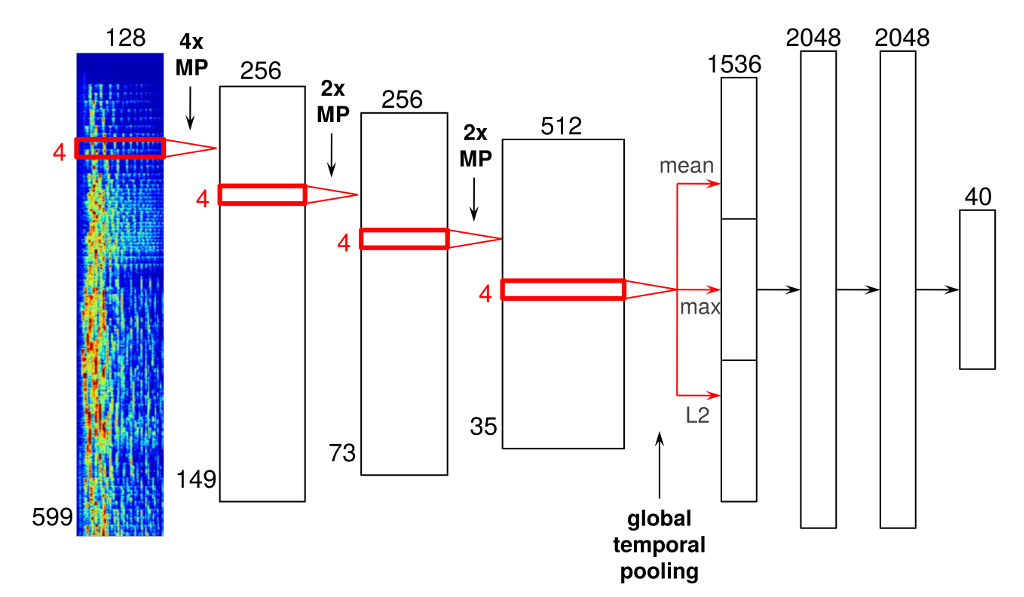
\includegraphics[scale=1.5]{img/rconv}
		\end{center}
\end{frame}

\begin{frame}{General scheme, what did we do?} 	
	\begin{center}				
		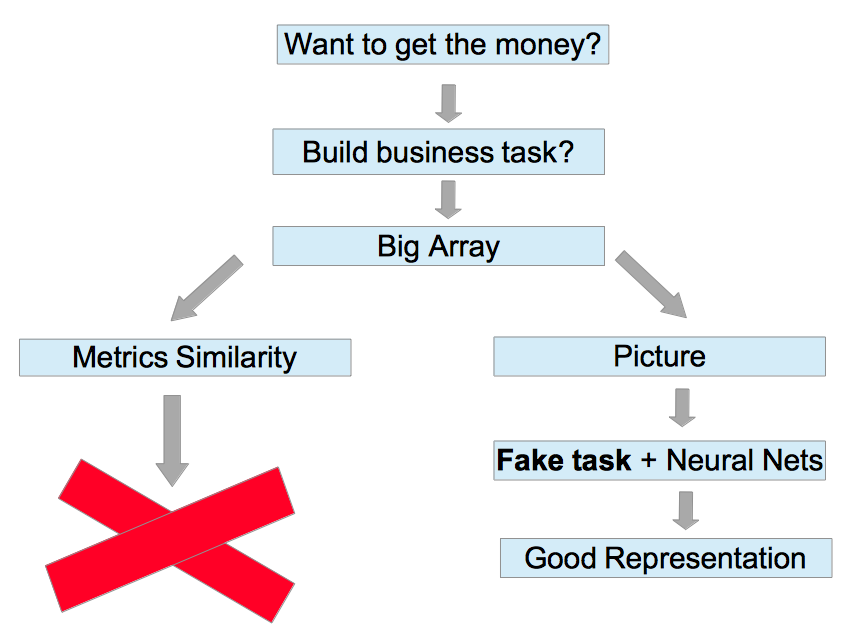
\includegraphics[scale=0.3]{img/scheem}
	\end{center}
\end{frame}

\begin{frame}{How to measure quality of good representation?} 
	What do we have?
	\begin{itemize}
		\item We have had represented each track as a vector
		\item But maybe our solution is too bad, how can we understand that?
		\item How to test "good representation"?
	\end{itemize}
	
	Let's invent the metrics:
		\begin{itemize}
			\item using assessors
			\item recommendation quality 
			\item using vectors to classify another labels
		\end{itemize}
\end{frame}

\begin{frame}{Let's adapt to Different length and Additional information} 
	How to use any length?:
		\begin{enumerate}
			\item Average prediction for many patches 		
			\item Recurrent neural net on many patches
				\begin{center}				
					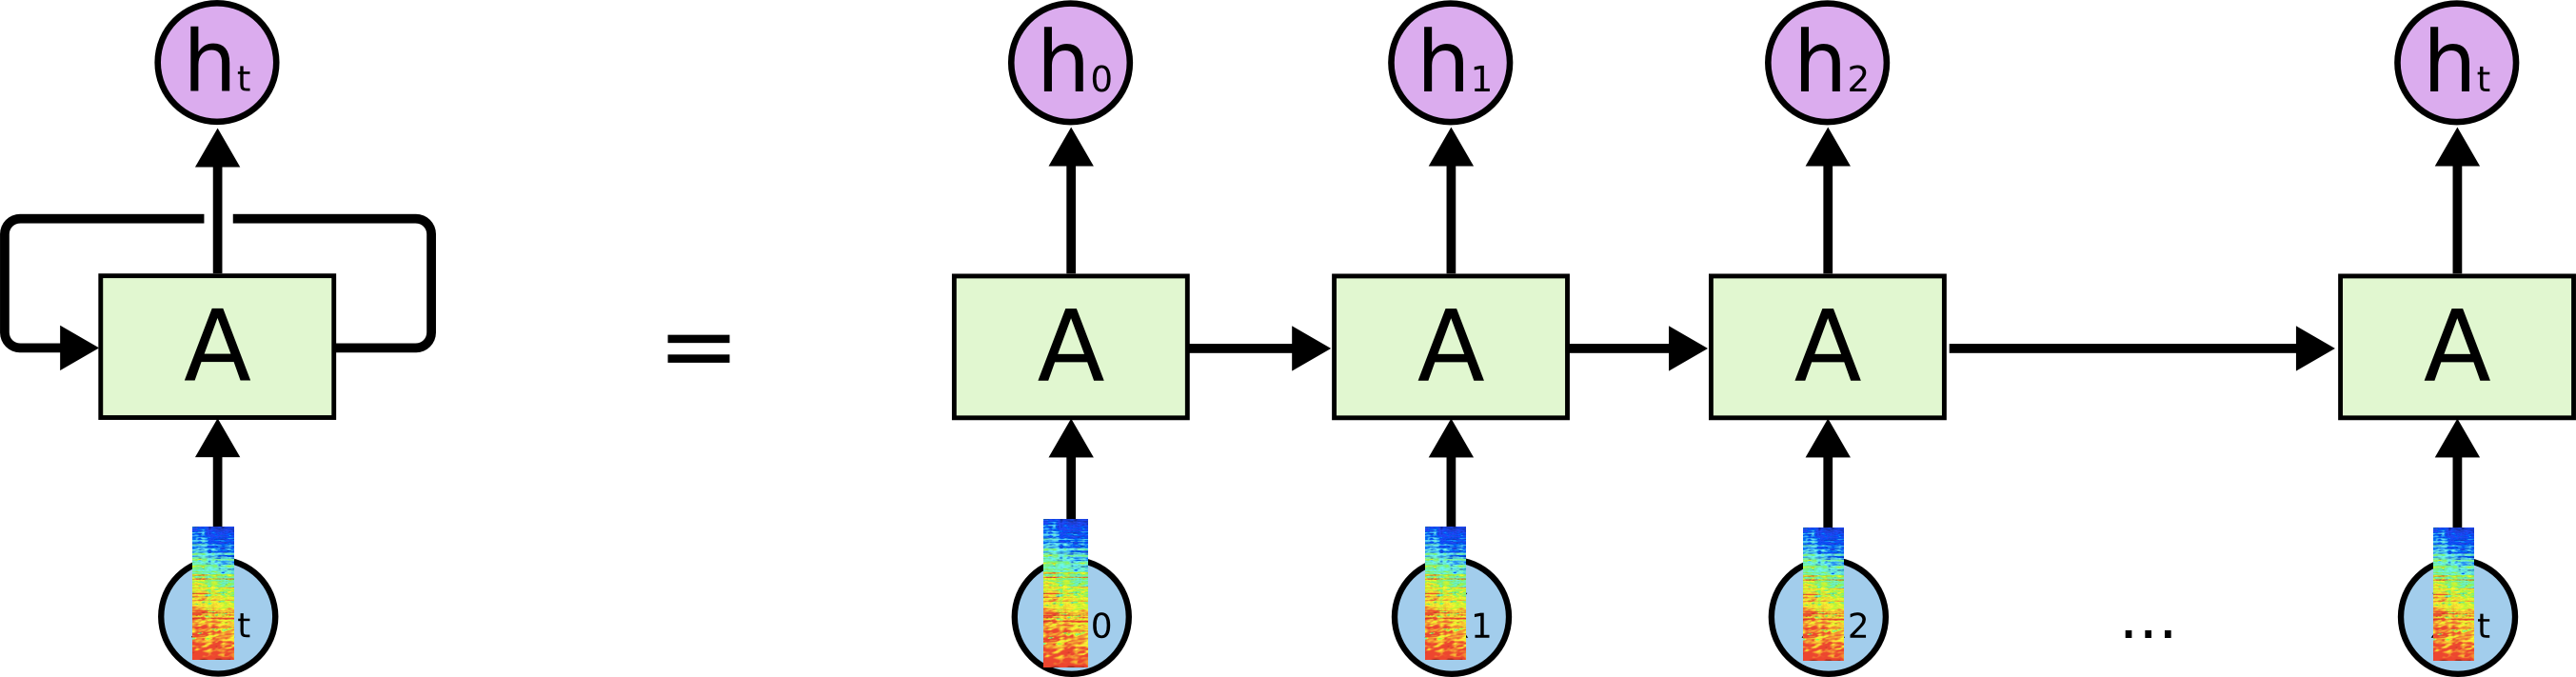
\includegraphics[scale=0.25]{img/rnn}
				\end{center} 
			\item Whatever?
		\end{enumerate}
	How to take account?:
		\begin{enumerate}
			\item Lyrics
				\begin{center}
					Concat(TextRNN, Conv) $\rightarrow$ FC $\rightarrow$ Cost
				\end{center}
			\item Genre, Artist, Year -- embedding too, multi-cost task
			\item ....
		\end{enumerate}
\end{frame}

\begin{frame}{Technical details} 
	How to build fast system for million users?
	\begin{enumerate}
		\item pre-compute vectors and tracks simulation 
		\item fast key-value storage
	\end{enumerate}
		\begin{center}				
			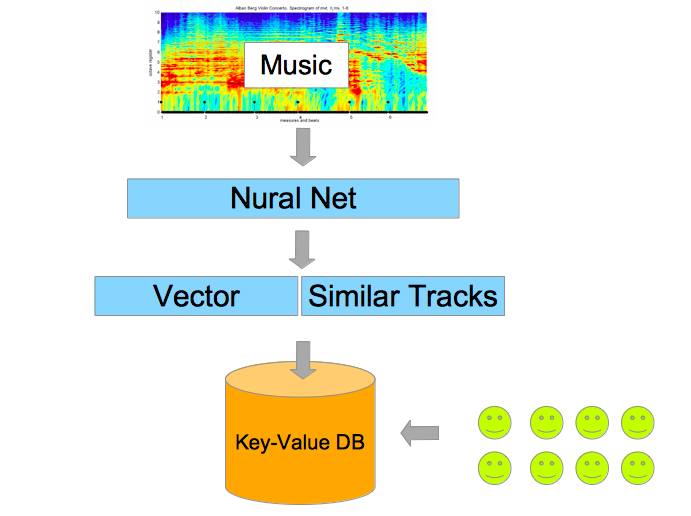
\includegraphics[scale=0.35]{img/prod}
		\end{center}
\end{frame}
	
\begin{frame}{End} 
	\begin{center}				
		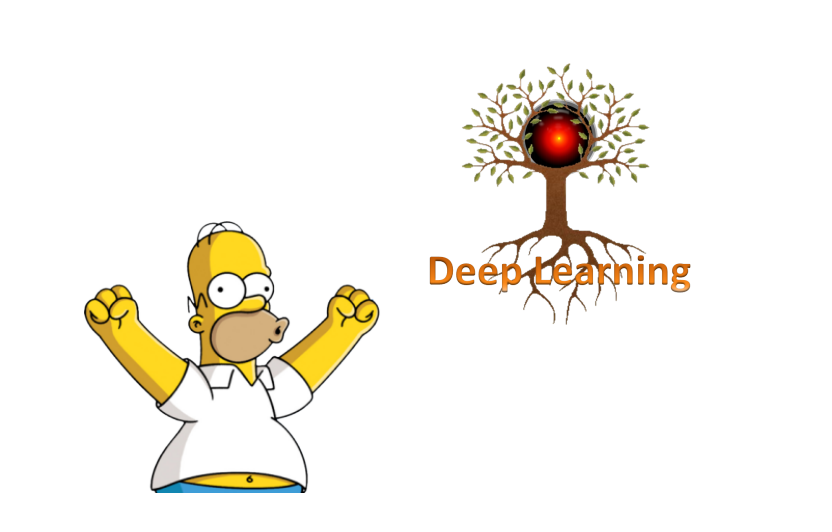
\includegraphics[scale=0.35]{img/csf}
	
		{\huge Current Status of your Field!}
		
		Thanks for your attention!
	\end{center}
\end{frame}

\end{document}

